\documentclass{article}

\usepackage{ragged2e}
\usepackage{graphicx}
\usepackage{amsmath}
\usepackage{siunitx}
\usepackage{hyperref}

% This stuff is for figures, don't copy-paste
\usepackage{float}
\DeclareGraphicsExtensions{.png, .pdf}
%\DeclareGraphicsExtensions{.pdf, .png}

\renewcommand{\c}[1]{\texttt{#1}}

\begin{document}

%\begin{flushright}
    \noindent
    Rodrigo Becerril Ferreyra\\
    E E 381 Section 12\\
    Lab 2\\
    02 October 2020
%\end{flushright}

\addcontentsline{toc}{section}{Introduction}
\section*{Introduction} The purpose of this lab is to practice
conditional probability using Python. The background situation
for all four Problems is the following: we are trying to
send a message in binary through a noisy channel, where there
is a probability of an individual bit being received as a 0
instead of a 1, or a 1 instead of a 0.

We define the random variables \(S\) and \(R\)
referring to the sent bit and the received bit, respectively,
where \(P(S = 0) = p_0\), \(P(S = 1) = p_1\),
and \(P\) is the probability function. All
Problems respect the following constants:
\begin{itemize}
    \item The probability that a 0 will be sent \(p_0 = 0.6\)
    \item The probability that a 1 will be sent
    \(p1 = 1-p_0 = 0.4\)
    \item The probability that a sent 0 will be received as
    a 1 \(\varepsilon_0 = 0.05\)
    \item The probability that a sent 1 will be received as
    a 0 \(\varepsilon_1 = 0.03\)
\end{itemize}

An image displaying the raw output of the Python source file
can be found at the end of this document.

\section{Problem 1}
\subsection{Question} The purpose of this Problem is to find
\(P(S \ne R)\), that being the probability of not receiving the
same bit that was sent: if the sent bit is 0 and the received
bit is 0, or if the sent bit is 1 and the received bit is 1,
then the experiment is considered a success; if the two bits
do not match, then it is not a success---the task is to
find the ratio of non-successes to the total number of
bits sent. For this experiment, \num{100000} bits were sent.

\subsection{Results} Out of the \num{100000} bits, \num{95703}
bits were sent successfully, which means that
\(\num{100000} - \num{95703} = \num{4297}\) bits were received
erroneously. This is a probability of \(0.04297\).

Table 1
displays the results of this experiment. Note that this
experiment took about \SI{0.556}{\second}.

\begin{table}[H]
    \centering\begin{tabular}{| r | l |}
        \hline
        Probability of transmission error & \\ \hline
        Ans. & \(p = 0.04297\) \\ \hline
    \end{tabular}
    \caption{Results of Problem 1.}
    \label{table:prob1}
\end{table}

\section{Problem 2}
\subsection{Question} The purpose of this Problem is to find
\(P(R = 1 \mid S = 1)\), that being the probability of
receiving a 1 with the knowledge that the sent bit is also a 1.
This is also known as the conditional probability of
\(R = 1\) given \(S = 1\). Again, \num{100000} bits were sent
in this experiment.

\subsection{Results} Out of the \num{100000} bits that were
sent,
only \num{39876} of them
were 1. Of these \num{39876} bits, \num{38636} were received
as a 1. This makes the probability
\(P(R = 1 \mid S = 1) = \num{38636}/\num{39876} = 0.96890\).

Table 2 shows the results of this experiment.
Note that this experiment took about \SI{0.545}{\second}.

\begin{table}[H]
    \centering\begin{tabular}{|r | l |}
        \hline
        Conditional probability \(P(R = 1 \mid S = 1)\) & \\ \hline
        Ans. & \(p = 0.96890\) \\ \hline
    \end{tabular}
    \caption{Results of Problem 2.}
    \label{table:prob2}
\end{table}

\section{Problem 3}
\subsection{Question} The purpose of this Problem is to find
\(P(S = 1 \mid R = 1)\), that being the probability that,
knowing that you received a 1, a 1 was sent. \num{100000}
bits were sent in this experiment.

\subsection{Results} Out of \num{100000} bits, \num{41642}
were received as 1, and \num{38616} of \textit{those}
were sent as 1. This means that \num{3026} bits were
erroneously received as 1. This means that
\(P(S=1\mid R=1) = \num{38616}/\num{41642} = 0.92733\).

Table 3 displays the results of this experiment. Note that this
experiment took about \SI{0.365}{\second}.

\begin{table}[H]
    \centering\begin{tabular}{| r | l |}
        \hline
        Conditional probability \(P(S = 1 \mid R = 1)\) & \\ \hline
        Ans. & \(p = 0.92733\) \\ \hline
    \end{tabular}
    \caption{Results of Problem 3.}
    \label{table:prob3}
\end{table}

\section{Problem 4}
\subsection{Question} The purpose of this Problem is to
verify whether a redundancy approach to the problem of
sending bits through a noisy channel is effective. In this
experiment, the same bit is sent three times (and received
three times). The three received bits are then fed into
a three-input majority rule circuit, whose truth table is
detailed below.

\begin{table}[H]
    \centering\begin{tabular}{c | c | c || c}
        \c{R3} & \c{R2} & \c{R1} & \c{D} \\ \hline
        0 & 0 & 0 & 0 \\ \hline
        0 & 0 & 1 & 0 \\ \hline
        0 & 1 & 0 & 0 \\ \hline
        0 & 1 & 1 & 1 \\ \hline
        1 & 0 & 0 & 0 \\ \hline
        1 & 0 & 1 & 1 \\ \hline
        1 & 1 & 0 & 1 \\ \hline
        1 & 1 & 1 & 1 \\
    \end{tabular}
    \caption{The truth table for a three-input majority rule circuit.}
    \label{table:majority}
\end{table}

D becomes the new ``received bit.''
If D is the same as the sent bit S, then the send is successful.
\num{100000} bits were sent in this experiment. In this
Problem, the task is to find the probability that a bit
will be sent incorrectly.

\subsection{Results} Out of the \num{100000} sends,
\num{99455} were decoded correctly (the decoded value D
was the same as the sent bit S), so \num{545} sends were
decoded incorrectly. The probability of receiving an
incorrect bit is \(p = \num{545}/\num{100000} = 0.00545\).

It is worth noting that this probability
of failure
is significantly smaller than the probability of failure
calculated in Problem 1 (\(0.04297\)), by one order of
magnitude. This means that sending redundant bits
and decoding them at the point of arrival is worth the
extra effort, because there is a smaller chance that
the sent bit will be received incorrectly.

Table 5 displays the results of this experiment. Note that
this experiment took about \SI{0.912}{\second}.

\begin{table}[H]
    \centering\begin{tabular}{| r | l |}
        \hline
        Probability of error with enhanced transmission & \\ \hline
        Ans. & \(p = 0.00545\) \\ \hline
    \end{tabular}
    \caption{Results of Problem 4}
    \label{table:prob4}
\end{table}

\pagebreak

\section{Output of Source File}
\begin{figure}[H]
    \centering
    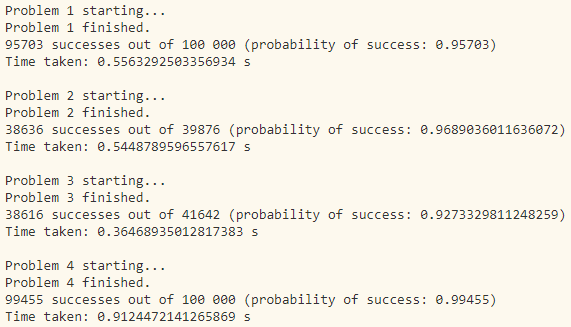
\includegraphics[width=\textwidth]{Images/output}
    \label{output}
\end{figure}

\end{document}
